\documentclass[12pt]{report}
\usepackage[utf8]{inputenc}
\usepackage[russian]{babel}
%\usepackage[14pt]{extsizes}
\usepackage{listings}
\usepackage{graphicx}
\usepackage{amsmath,amsfonts,amssymb,amsthm,mathtools} 
\usepackage{pgfplots}
\usepackage{filecontents}
\usepackage{indentfirst}
\usepackage{eucal}
\usepackage{enumitem}
\frenchspacing

\usepackage{indentfirst} % Красная строка


\usetikzlibrary{datavisualization}
\usetikzlibrary{datavisualization.formats.functions}

\usepackage{amsmath}




% Для листинга кода:
\lstset{ %
language=C++,                 % выбор языка для подсветки (здесь это С++)
basicstyle=\small\sffamily, % размер и начертание шрифта для подсветки кода
numbers=left,               % где поставить нумерацию строк (слева\справа)
numberstyle=\tiny,           % размер шрифта для номеров строк
stepnumber=1,                   % размер шага между двумя номерами строк
numbersep=5pt,                % как далеко отстоят номера строк от подсвечиваемого кода
showspaces=false,            % показывать или нет пробелы специальными отступами
showstringspaces=false,      % показывать или нет пробелы в строках
showtabs=false,             % показывать или нет табуляцию в строках
frame=single,              % рисовать рамку вокруг кода
tabsize=2,                 % размер табуляции по умолчанию равен 2 пробелам
captionpos=t,              % позиция заголовка вверху [t] или внизу [b] 
breaklines=true,           % автоматически переносить строки (да\нет)
breakatwhitespace=false, % переносить строки только если есть пробел
escapeinside={\#*}{*)}   % если нужно добавить комментарии в коде
}

\usepackage[left=2cm,right=2cm, top=2cm,bottom=2cm,bindingoffset=0cm]{geometry}
% Для измененных титулов глав:
\usepackage{titlesec, blindtext, color} % подключаем нужные пакеты
\definecolor{gray75}{gray}{0.75} % определяем цвет
\newcommand{\hsp}{\hspace{20pt}} % длина линии в 20pt
% titleformat определяет стиль
\titleformat{\chapter}[hang]{\Huge\bfseries}{\thechapter\hsp\textcolor{gray75}{|}\hsp}{0pt}{\Huge\bfseries}


% plot
\usepackage{pgfplots}
\usepackage{filecontents}
\usetikzlibrary{datavisualization}
\usetikzlibrary{datavisualization.formats.functions}

\begin{document}
%\def\chaptername{} % убирает "Глава"
\thispagestyle{empty}
\begin{titlepage}
	\noindent \begin{minipage}{0.15\textwidth}
	
\includegraphics[width=\linewidth]{report_files/bmstu_logo.jpg}
	\end{minipage}
	\noindent\begin{minipage}{0.9\textwidth}\centering
		\textbf{Министерство науки и высшего образования Российской Федерации}\\
		\textbf{Федеральное государственное бюджетное образовательное учреждение высшего образования}\\
		\textbf{~~~«Московский государственный технический университет имени Н.Э.~Баумана}\\
		\textbf{(национальный исследовательский университет)»}\\
		\textbf{(МГТУ им. Н.Э.~Баумана)}
	\end{minipage}
	
	\noindent\rule{18cm}{3pt}
	\newline\newline
	\noindent ФАКУЛЬТЕТ $\underline{\text{«Информатика и системы управления»}}$ \newline\newline
	\noindent КАФЕДРА $\underline{\text{«Программное обеспечение ЭВМ и информационные технологии»}}$\newline\newline\newline\newline\newline
	
	
	\begin{center}
		\noindent\begin{minipage}{1.3\textwidth}\centering
			\Large\textbf{  Отчет по лабораторной работе №4}\newline
			\textbf{по дисциплине "Анализ алгоритмов"}\newline\newline
		\end{minipage}
	\end{center}
	
	\noindent\textbf{Тема} $\underline{\text{Многопоточность на CUDA}}$\newline\newline
	\noindent\textbf{Студент} $\underline{\text{Костев Д.И.}}$\newline\newline
	\noindent\textbf{Группа} $\underline{\text{ИУ7-51Б}}$\newline\newline
	\noindent\textbf{Оценка (баллы)} $\underline{\text{~~~~~~~~~~~~~~~~~~~~~~~~~~~}}$\newline\newline
	\noindent\textbf{Преподаватели} $\underline{\text{Волкова Л.Л. }}$\newline\newline\newline
	
	\begin{center}
		\vfill
		Москва~---~\the\year
		~г.
	\end{center}
\end{titlepage}

\setcounter{page}{2}
\tableofcontents

\newpage
\chapter*{Введение}
\addcontentsline{toc}{chapter}{Введение}
Многопоточность — способность центрального процессора (CPU) или одного ядра в многоядерном процессоре одновременно выполнять несколько процессов или потоков, соответствующим образом поддерживаемых операционной системой.

Этот подход отличается от многопроцессорности, так как многопоточность процессов и потоков совместно использует ресурсы одного или нескольких ядер: вычислительных блоков, кэш-памяти ЦПУ или буфера перевода с преобразованием (TLB).


В тех случаях, когда многопроцессорные системы включают в себя несколько полных блоков обработки, многопоточность направлена на максимизацию использования ресурсов одного ядра, используя параллелизм на уровне потоков, а также на уровне инструкций.

Поскольку эти два метода являются взаимодополняющими, их иногда объединяют в системах с несколькими многопоточными ЦП и в ЦП с несколькими многопоточными ядрами.


Многопоточная парадигма стала более популярной с конца 1990-х годов, поскольку усилия по дальнейшему использованию параллелизма на уровне инструкций застопорились.

Смысл многопоточности — квазимногозадачность на уровне одного исполняемого процесса.

Значит, все потоки процесса помимо общего адресного пространства имеют и общие дескрипторы файлов. Выполняющийся процесс имеет как минимум один (главный) поток.


Многопоточность (как доктрину программирования) не следует путать ни с многозадачностью, ни с многопроцессорностью, несмотря на то, что операционные системы, реализующие многозадачность, как правило, реализуют и многопоточность.


Достоинства:

\begin{itemize}

	\item облегчение программы посредством использования общего адресного пространства;

	\item меньшие затраты на создание потока в сравнении с процессами;

	\item повышение производительности процесса за счёт распараллеливания процессорных вычислений;

	\item если поток часто теряет кэш, другие потоки могут продолжать использовать неиспользованные вычислительные ресурсы.

\end{itemize}


Недостатки:

\begin{itemize}

	\item несколько потоков могут вмешиваться друг в друга при совместном использовании аппаратных ресурсов;

	\item с программной точки зрения аппаратная поддержка многопоточности более трудоемка для программного обеспечения;

	\item проблема планирования потоков;

	\item специфика использования. Вручную настроенные программы на ассемблере, использующие расширения MMX или AltiVec и выполняющие предварительные выборки данных, не страдают от потерь кэша или неиспользуемых вычислительных ресурсов. Таким образом, такие программы не выигрывают от аппаратной многопоточности и действительно могут видеть ухудшенную производительность из-за конкуренции за общие ресурсы.

\end{itemize}

Однако несмотря на количество недостатков, перечисленных выше, многопоточная парадигма имеет большой потенциал на сегодняшний день и при должном написании кода позволяет значительно ускорить однопоточные алгоритмы.

\section*{Цель лабораторной работы}
Целью данной лабораторной работы является изучение и реализация параллельных вычислений.

\section*{Задачи лабораторной работы}
\indent В рамках выполнения работы необходимо решить следующие задачи:

\begin{itemize}

	\item изучить понятие параллельных вычислений;

	\item реализовать последовательный и  параллельный реализации алгоритма перемножения матриц(на GPU);

	\item сравнить временные характеристики реализованных алгоритмов экспериментально.
\end{itemize}

\chapter{Аналитическая часть}

\section{Описание задачи}


Пусть даны две прямоугольные матрицы
\begin{equation}
A_{lm} = \begin{pmatrix}
a_{11} & a_{12} & \ldots & a_{1m}\\
a_{21} & a_{22} & \ldots & a_{2m}\\
\vdots & \vdots & \ddots & \vdots\\
a_{l1} & a_{l2} & \ldots & a_{lm}
\end{pmatrix},
\quad
B_{mn} = \begin{pmatrix}
b_{11} & b_{12} & \ldots & b_{1n}\\
b_{21} & b_{22} & \ldots & b_{2n}\\
\vdots & \vdots & \ddots & \vdots\\
b_{m1} & b_{m2} & \ldots & b_{mn}
\end{pmatrix},
\end{equation}
тогда матрица $C$
\begin{equation}
C_{ln} = \begin{pmatrix}
c_{11} & c_{12} & \ldots & c_{1n}\\
c_{21} & c_{22} & \ldots & c_{2n}\\
\vdots & \vdots & \ddots & \vdots\\
c_{l1} & c_{l2} & \ldots & c_{ln}
\end{pmatrix},
\end{equation}
где
\begin{equation}
\label{eq:M}
c_{ij} =
\sum_{r=1}^{m} a_{ir}b_{rj} \quad (i=\overline{1,l}; j=\overline{1,n})
\end{equation}
будет называться произведением матриц $A$ и $B$.


В данной лабораторной работе стоит задача распараллеливания алгоритма Винограда по 2 схемам. Так как каждый элемент матрицы $C$ вычисляется независимо от других и матрицы $A$ и $B$ не изменяются, то для параллельного вычисления произведения, достаточно просто равным образом распределить элементы матрицы $C$ между потоками.



\section{Вывод}
	Обычный алгоритм перемножения матриц независимо вычисляет элементы матрицы-результата, что дает большое количество возможностей для реализации параллельного варианта алгоритма.
\clearpage


\chapter{Конструкторская часть}
\section{Схемы алгоритмов}
На рисунке 2.1 представлена схема обычного алгоритма перемножения матриц (без распараллеливания). На рисунке 2.2 представлена схема распараллеливания алгоритма умножения матриц.


\begin{figure}[hp!]
	\centering
	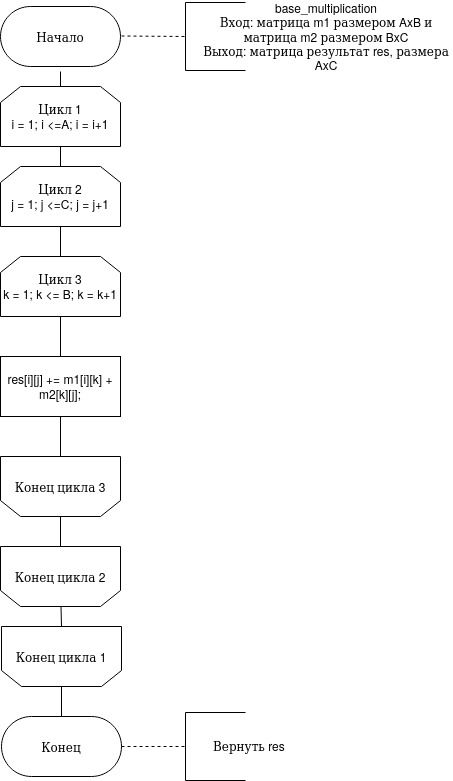
\includegraphics[scale=0.5]{report_files/base.jpg}
	\caption{Схема стандартного алгоритма умножения матриц.}
	\label{fig:mpr}
\end{figure}
\newpage
На рисунке 2.3 представленна схема с параллельным выполнением цикла (по строкам матрицы).
\begin{figure}[hp!]
	\centering
	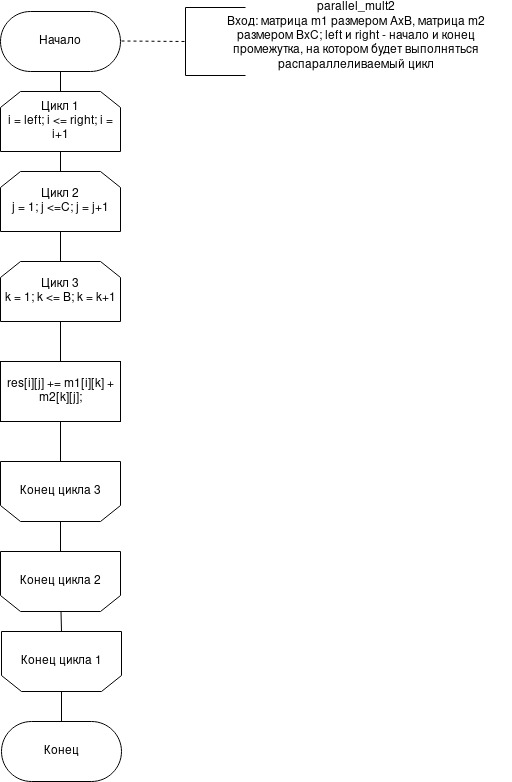
\includegraphics[scale=0.7]{report_files/parallel1.jpg}
	\caption{Схема распараллеленного алгоритма умножения матриц, способ №1.}
	\label{fig:mpr}
\end{figure}

\newpage
\begin{figure}[hp!]
	\centering
	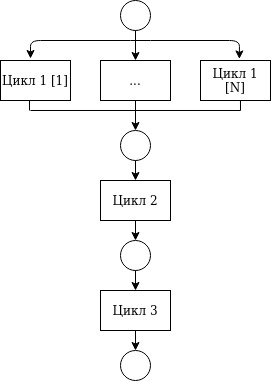
\includegraphics[scale=0.7]{report_files/parallel_scheme.jpg}
	\caption{Схема с параллельным выполнением первого цикла}
	\label{fig:mpr}
\end{figure}


\section{Вывод}
На основе теоретических данных, полученных из аналитического раздела, была построена схема стандартного алгоритма умножения матриц, а так же после разделения алгоритма на этапы были предложены 2 схемы параллельного выполнения данных этапов.

\chapter{Технологическая часть}

В данном разделе приведены средства реализации и листинги кода.

\section{Требование к ПО}

К программе предъявляется ряд требований:

\begin{itemize}
	\item на вход подаются размеры 2 матриц, а также их элементы;
	\item на выходе — матрица, которая является результатом умножения входных матриц.
\end{itemize}

\section{Средства реализации}
Для реализации ПО я выбрал язык программирования Сuda. Данный выбор обусловлен высокой скоростью работы языка, а так же наличия инструментов для создания и эффективной работы с потоками.

\section{Реализация алгоритмов}

В листингах 3.1 - 3.2 приведена реализация расмотренных ранее алгоритмов перемножения матриц.

\begin{lstlisting}[label=some-code,caption=Функция умножения матриц обычным способом, language=C]
__global__ void matmulsimp(int* M, int* N, int* P, int width) {
	for (int row = 0; row < width; row++) {
		for (int col = 0; col < width; col++) {
			// Multiply the row of A by the column of B to get the row, column of product.
			for (int inner = 0; inner < width; inner++)
				P[row * width + col] += M[row * width + inner] * N[inner * width + col];
		}
	}
}
\end{lstlisting}
\newpage
\begin{lstlisting}[label=some-code,caption=Функция умножения матриц параллельно,language=C]
__global__ void MatMul(int* M, int* N, int* P, int width)
{
	int x = threadIdx.x;
	int y = threadIdx.y;

	float Pervalue = 0;

	float elem1 = 0.0, elem2 = 0.0, value = 0.0;
	for (int i = 0; i < width; i++)
	{
		elem1 = M[y * width + i]; // Возьмем одну строку матрицы M
		elem2 = N[i * width + x]; // Берем один столбец из N матрицы

		value += elem1 * elem2; // Сумма
	}

	P[y * width + x] = value;
}
\end{lstlisting}

\section{Тестовые данные}

В таблице~\ref{tabular:test_rec} приведены тесты для функций, реализующих параллельное и обычное умножение матриц. Все тесты пройдены успешно.

\begin{table}[h!]
	\begin{center}
	    \caption{\label{tabular:test_rec} Тестирование функций}
		\begin{tabular}{c@{\hspace{7mm}}c@{\hspace{7mm}}c@{\hspace{7mm}}c@{\hspace{7mm}}c@{\hspace{7mm}}c@{\hspace{7mm}}}
			\hline
			Первая матрица & Вторая матрица & Ожидаемый результат \\ \hline
			\vspace{4mm}
			$\begin{pmatrix}
			1 & 2 & 3\\
			1 & 2 & 3\\
			1 & 2 & 3
			\end{pmatrix}$ &
			$\begin{pmatrix}
			1 & 2 & 3\\
			1 & 2 & 3\\
			1 & 2 & 3
			\end{pmatrix}$ &
			$\begin{pmatrix}
			6 & 12 & 18\\
			6 & 12 & 18\\
			6 & 12 & 18
			\end{pmatrix}$ \\
			\vspace{2mm}
			\vspace{2mm}
			$\begin{pmatrix}
			1 & 2 & 2\\
			1 & 2 & 2
			\end{pmatrix}$ &
			$\begin{pmatrix}
			1 & 2\\
			1 & 2\\
			1 & 2
			\end{pmatrix}$ &
			$\begin{pmatrix}
			5 & 10\\
			5 & 10
			\end{pmatrix}$ \\
			\vspace{2mm}
			\vspace{2mm}
			$\begin{pmatrix}
			2
			\end{pmatrix}$ &
			$\begin{pmatrix}
			2
			\end{pmatrix}$ &
			$\begin{pmatrix}
			4
			\end{pmatrix}$ \\
			\vspace{2mm}
			\vspace{2mm}
			$\begin{pmatrix}
			1 & -2 & 3\\
			1 & 2 & 3\\
			1 & 2 & 3
			\end{pmatrix}$ &
			$\begin{pmatrix}
			-1 & 2 & 3\\
			1 & 2 & 3\\
			1 & 2 & 3
			\end{pmatrix}$ &
			$\begin{pmatrix}
			0 & 4 & 6\\
			4 & 12 & 18\\
			4 & 12 & 18
			\end{pmatrix}$\\
			\vspace{2mm}
			\vspace{2mm}
		\end{tabular}
	\end{center}
\end{table}

\section{Вывод}

В данном разделе были разработаны исходные коды алгоритмов: обычный способ умножения матриц и два способа параллельного перемножения матриц.


\chapter{Исследовательская часть}

\section{Технические характеристики}

Ниже приведеные технические характеристики устройства, на котором было проведенно тестирование ПО.

\begin{itemize}

	\item Операционная система: Windows 11 64-bit.

	\item Оперативная память: 8 ГБ.

	\item Процессор: Intel(R) Core(TM) i5-8250 CPU @ 1.60ГГц.

\end{itemize}

\section{Время выполнения алгоритмов}

В таблице 4.1 представлены замеры времени работы для каждого из алгоритмов на разных размерах матриц.

\begin{table} [h!]
	\caption{Таблица времени выполнения алгоритмов(в милисекундах)}
	\begin{center}
		\begin{tabular}{|c c c|} 
		 	\hline
			Размер матрицы & Cuda & Cтандарт \\  
			\hline
            3 & 1.157120 & 0.141376 \\ 
            \hline
            10 & 0.527360 & 1.644640 \\ 
            \hline
            20 & 0.097280 & 13.453536 \\ 
            \hline
            30 &  0.116768 & 39.8552320 \\ 
            \hline
            40 & 1.094656 & 93.969246 \\ 
            \hline
            50 & 0.226304 & 188.345596 \\ 
            \hline
            100 & 0.013312 & 1408.762817 \\ 
            \hline
            200 & 0.021056 & 9884.333984 \\ 
            \hline
		\end{tabular}
	\end{center}
\end{table}

\section{Вывод}
При малых размерах матриц различия времени - минимальны, из-за того что часть времени, в которой выигрывает параллельная реализация, тратится на распределение потоков. Но при больших размерах становится видно, что скорость параллельной реализации на Сuda куда выше. Так при 200 элементах скорость параллельногой реализации в 470000 раз выше.

\chapter*{Заключение}
\addcontentsline{toc}{chapter}{Заключение}

В рамках данной лабораторной работы была достигнута её цель: изучены паралелльные вычисления. Также выполнены следующие задачи:

\begin{itemize}
	\item было изучено понятие параллельных вычислений;
	\item были реализованы обычный и параллельный реализаций алгоритма перемножения матриц;
	\item было произведено сравнение временных характеристик реализованных алгоритмов экспериментально.
\end{itemize}

Параллельные реализации алгоритмов выигрывают по скорости у обычной (однопоточной) реализации перемножения двух матриц. Наиболее эффективны данные алгоритмы при количестве потоков, совпадающем с количеством логических ядер компьютера. Потому что задействован каждый поток.


\newpage
\addcontentsline{toc}{chapter}{Литература}
\begin{thebibliography}{}
\bibitem{bibKormen}
Кормен Т. Алгоритмы: построение и анализ [Текст] / Корм ен Т. - Вильямс, 2014. - 198 с. - 219 с.
\bibitem{bibGetProcessTimes}
GetProcessTimes function. URL: https://docs.microsoft.com/en-us/windows/win32/api/processthreadsapi/nf-processthreadsapi-getprocesstimes, 01.10.2021
\bibitem{bibwiki}
Алгоритм Копперсмита — Винограда. URL: https://ru.wikipedia.org/wiki/Алгоритм-Копперсмита—Винограда
\end{thebibliography}
	
\bibliographystyle{utf8gost705u}  % стилевой файл для оформления по ГОСТу


\end{document} 